\documentclass[11]{article}

\usepackage[backend=bibtex]{biblatex}
\bibliography{references}

\usepackage{graphicx}
\usepackage{hyperref}
\hypersetup{colorlinks,urlcolor=blue}

\usepackage{listings}
\usepackage{xcolor}
\definecolor{darkgray}{rgb}{.35,.25,.35}
\definecolor{lightgray}{rgb}{.6,.6,.6}

%\lstdefinelanguage{bash}{
%  keywords={git,update,apt-get,submodule,init,clone},
%  keywordstyle=\color{cyan}\bfseries,
%  ndkeywords={return, null},
%  ndkeywordstyle=\color{red}\bfseries,
%  identifierstyle=\color{darkgray},
%  sensitive=false,
%  comment=[l]{//},
%  morecomment=[s]{/*}{*/},
%  commentstyle=\color{lightgray}\ttfamily,
%  stringstyle=\color{red}\ttfamily,
%  morestring=[b]',
%  morestring=[b]"
%}
\lstdefinelanguage{bash}{
  basicstyle=\scriptsize\ttfamily\color{white},
  backgroundcolor=\color{lightgray},
  commentstyle = \color{darkgray},
  keywordstyle = \color{white},
  rulecolor    = \color{black},
  stringstyle  = \color{white}
  commentstyle=\color{lightgray}\ttfamily
}

\lstset{
   language=bash,
   extendedchars=true,
   basicstyle=\scriptsize\ttfamily,
   showstringspaces=false,
   showspaces=false,
   tabsize=2,
   showtabs=false,
   captionpos=b,
}


\begin{document}

\section{Review : Contour Matching Techniques}

\subsection{Motivation}
In optimising our tool positional search, we can determine the regions of contact that are more likely to be good fit for the active and passive object interaction. This follows the ideas proposed by \cite{battaglia2013}, in that humans build mental models of objects to allow inference over  the physical world. Human subjects would therefore have understanding of the geometric constraints of the physical world and of the forces generated by their actions.

Interaction with a high likelihood for success would have to satisfy two criteria: 
\begin{enumerate}
\item \textbf{Geometric constraints} of the two objects must be met ( i.e. the shapes of the two objects should adequately fit )
\item \textbf{Contact forces} generated must correspond to the intention of the actions executed (i.e. for a lifting action, the human subject would focus on points of interaction that would permit vertical forces to be applied)
\end{enumerate}

The total space of possible solutions can be reduced by these criteria without explicit simulation (akin mental simulations\cite{osiurak2014}). The physics engine would later verify the potential of different solutions. 

\subsection{Geometric Constraints}
The geometries of the tool and object must be compatible. In other words, either the active or passive object's geometry must fit within the gaps and edges of its counterpart. Tighter fits, offer better transfer of energy and control over the movement of the passive object. A better fit would therefore require less manipulation effort. In the paradigm of 4CT \cite{osiurak2014}, the effort constraint may explain user's preference for one geometric solution over another.

It is not necessary for the whole geometry of objects to fit. It is sufficient for the tool to have the necessary parts acting as affordance and functional basis (end effector\cite{zhu2015}). If the functional part matches the gaps of the passive object, then the configuration is likely to achieve the desired effect. 

\subsubsection{Shape Description and Matching}

We consider techniques of shape similarity in matching object parts. Shape analysis techniques have traditionally been engaged in image processing and robot vision for detecting and tracking objects of similar features. The last two decades have provided many approaches for this type of problem \cite{loncaric1998,zhang2004,veltkamp2001,robert2012}. Fundamentally, the challenge lies in detecting similarity even as objects undergo geometric transformations (i.e. rotation,translation,scaling and shearing).     

Zhang\cite{zhang2004} et al. classify shape similarity into contour-based and region-based techniques. These are further divided into structural and global approaches. A comprehensive list and structure can be found in fig. \ref{fig:shape_similarity}.

\begin{figure}[h]
  \centering
  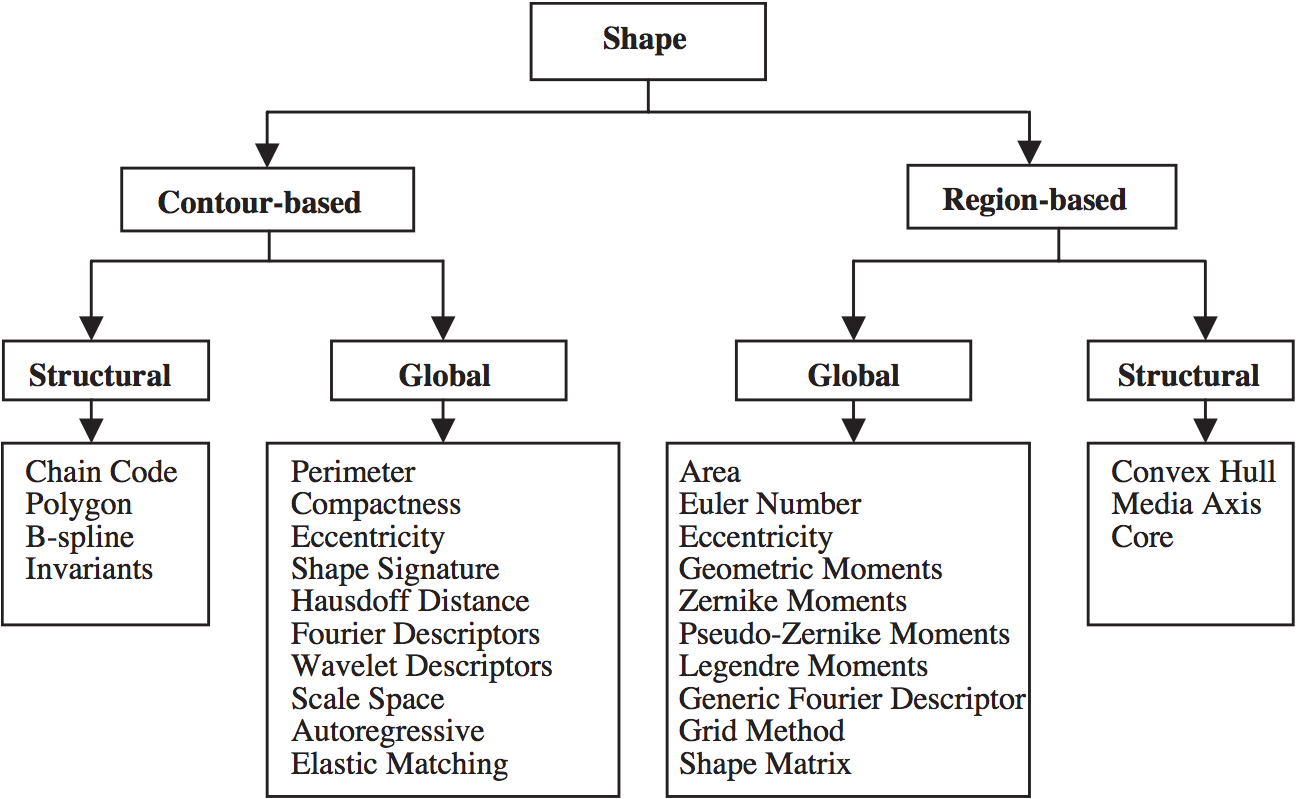
\includegraphics[width=1\textwidth]{./figures/similarity_techniques.png}
  \caption{Classification of shape similarity techniques (reprinted from \cite{zhang2004})}
  \label{fig:shape_similarity}
\end{figure}  

Contour techniques asses shape similarity by extracting features from the edge of detected objects. In comparison, region techniques work by assessing surface level information such as: colour features, gradient changes and surface medial. Techniques from both approaches have justification in human perception \cite{chatbri2016}. Nonetheless, our use case excludes most region-based approaches. Tool parts must correspond to shape gaps. It is hard to consider gaps as having the surface information needed for region-based matching.

In structural approaches, shapes are considered as composed out of primitives. In the case of contour techniques, primitives are segments on the boundary of an object. The organisation of primitives can be linear (feature vector\cite{zhang2004}) or hierarchical (tree like structures\cite{zhu2015}). Two objects are considered similar when they have the same primitive structures (or features). In comparison, global approaches make use of shapes as a whole when assessing similarity. 

Both structural and global approaches have justification in human perception \cite{zhang2004}. Human subjects show a preference for features even when other shape descriptors are available \cite{chatbri2016}. At the same time, global shape perception seems to preceed local feature detection\cite{navon1977}. 

Matching human behaviour requires more insight into human visual perception. Loncaric\cite{loncaric1998} describes some theories of human visual perception with interest in image processing. In a tool use scenario, emphasis should be given to theories describing perception as volumetric, such as through the use of generalised cylinders (geons\cite{dickinson2014}). Such insight may better explain human tool performance, but will however remain for future work.    

\subsubsection{Limitations}
As previously remarked, contour based techniques contain promising approaches for solving tool-object matching problems. It is important to consider some of the limitations of such techniques, especially with regards to human ability. 

Global contour matching techniques are sensitive to occlusion (i.e. part of the object is hidden from the view point by some obstacle). In such cases, structural approaches are better suited to identify shapes from visible parts. Human perception is regarded as able to recognise objects even from sparse information or occluded perspective \cite{loncaric1998}. In solving tool use scenarios, it is important to consider a subject's visual perspective ( point of view ). The geometry of objects may not be fully visible. 

Most shape similarity techniques are tailored to analysing image based information (i.e. 2D projections of reality). Human perception however also makes use of depth related knowledge. As tool use encompasses real world geometric constraints, any contour based approach would have to be adaptable to 3D information ( e.g. point clouds ). To simplify the problem of visual analysis, surface point coordinates are extracted directly from the physics simulator. 

We next consider a novel and simple approach for matching point surfaces. It avoids most of the problems enumerated above and scales well to multi-dimensional data.  



\section{Appendix 1 - Compilation}
The following section describes how to compile and run the computational model on Windows and Linux operating systems. 
Original source-code and documentation can be found at \url{https://github.com/iceiony/4ConstraintsTheory}
The below installation steps are meant to be run using a terminal window.

\subsection{Linux}
Linux and Unix based operating systems require GCC compiler version 4.6 or earlier. 
\begin{enumerate}
  \item Install \textbf{git} and clone the code repository: 
    \begin{lstlisting}[language=bash]
  apt-get update
  apt-get install git-core

  git clone https://github.com/iceiony/4ConstraintsTheory.git 
  cd 4ConstraintsTheory
  git submodule init
  git submodule update
    \end{lstlisting}

    If the folder ./ComputationalModel/newton-dynamics is missing, clone the physics engine repository:
    \begin{lstlisting}[language=bash]
  cd ./ComputationalModel
  git clone --depth 1 https://github.com/MADEAPPS/newton-dynamics.git 
    \end{lstlisting}

  \item Install \textbf{cmake version 3.2} (which is not available on Ubuntu by default): 
    \begin{lstlisting}[language=bash]
    apt-get install software-properties-common
    apt-get-repository ppa:george-edison55/cmake-3.x
    apt-get update
    apt-get install cmake
    \end{lstlisting}

  \item Install \textbf{GLFW3} library:
    \begin{lstlisting}[language=bash]
    add-apt-repository ppa:keithw/glfw3
    apt-get update
    apt-get install libglfw3
    apt-get install libglfw3-dev
    \end{lstlisting}

  \item Install \textbf{GLEW} library:
    \begin{lstlisting}[language=bash]
    apt-get install libglew-dev
    \end{lstlisting}
    

  \item Install \textbf{tinyxml} library:
    \begin{lstlisting}[language=bash]
    apt-get install libtinyxml-dev
    \end{lstlisting}
    
  \item The computational model source code is located in the ./ComputationalModel subfolder. To compile it run:
    \begin{lstlisting}[language=bash]
    cmake .
    make -j4
    \end{lstlisting}
\end{enumerate}

\subsection{Windows}
Windows based operating systems require the Visual C++ compiler which part of Visual Studio package.
The Windows solution contains pre-compiled packages required for graphic rendering. 
As these packages were compiled using VisualStudio - 2015, other viersions of the compiler would not work.   
\begin{enumerate}

  \item Install \textbf{git} using 
    \href{https://github.com/gitextensions/gitextensions/releases/latest}{GitExtensions-2.48-SetupComplete.msi} 
    During installation the following options should be chosen : 
    \begin{description}
	\item [MsysGit] should be installed 
	\item [OpenSSH] authentication should be chosen instead of Putty
    \end{description}

  \item After installation open \textbf{Git Bash} available in the start menu. Clone the code repository:   
    \begin{lstlisting}[language=bash]
  git clone https://github.com/iceiony/4ConstraintsTheory.git 
  cd 4ConstraintsTheory
  git submodule init
  git submodule update
    \end{lstlisting}

    If the folder ./ComputationalModel/newton-dynamics is missing, clone the physics engine repository:
    \begin{lstlisting}[language=bash]
  cd ./ComputationalModel
  git clone --depth 1 https://github.com/MADEAPPS/newton-dynamics.git 
    \end{lstlisting}

  \item Install \textbf{VisualStudio 2015} community edition, with the \textbf{Visual C++} option enabled. 
  
  \item Open the visual studio solution located in ./ComputationalModel/vs\_2015/ComputationalModel/ComputationalModel.sln. 
    Simply build any desired executable of the model.
    All output is directed to ./ComputationalModel/vs\_2015/ComputationalModel/bin . 

\end{enumerate}

Successful compilations would result in 4 executable files: 
\begin{itemize}
  \item ExhaustiveSearchGUI.exe 
  \item ExhaustiveSearch.exe
  \item ExtractSurfacePointsGUI.exe  
  \item VisualSearchGUI.exe
\end{itemize}

\section{Appendix 2 - Software Glossary}
This section describes the functional basis of the computational model software. 
For the graphic version of the software (files ending in GUI), camera view-point can be controlled using \textbf{W,A,S,D} keyboard keys and \textbf{Mouse Click \& Drag}.Execution of the 3D simulation can be paused and resumed by pressing the \textbf{P} key.

\begin{description}

  \item [ExhaustiveSearchGUI.exe] performs an exhaustive search of the tool and object fitting. It can be invoked from command line with the tool and object model files 	in 3DS file format. If no parameters are used, the executable will default to loading obj51.3ds and obj52.3ds .

    \begin{lstlisting}[language=bash]
  ./ExhaustiveSearchGUI.exe obj51.3ds obj52.3ds
    \end{lstlisting}

    On startup, the tool to object fitting is paused. Execution can be resumed and visualised in 3D by pressing the \textbf{'P'} key.
    Potential fitting position are written to \textbf{results.csv}.

  \item [ExhaustiveSearch.exe] performs an exhaustive search without the use of a graphic user interface. As no 3D rendering is shown, the execution is considerably faster. All output is written to \textbf{results.csv}

  \item [ExtractSurfacePointsGUI.exe] utility software for extracting points on the surface of an object in current view. The model of an object must be passed as parameter in 3DS format. 

    \begin{lstlisting}[language=bash]
  ./ExtractSurfacePointsGUI.exe obj51.3ds
    \end{lstlisting}

    Surface points are recorded every time physics simulation is paused (by hitting the \textbf{P} key).
    Output is written to the \textbf{./surfaces} subfolder with one file per extracted surface.   

  \item [VisualSearchGUI.exe] performs a visual search of surfaces that would potentially offer good tool to object interaction. Tool and object models can be passed as parameters. If the program is invoked with no arguments, obj51.3ds and obj52.3ds are loaded.
    
    \begin{lstlisting}[language=bash]
  ./VisualSearchGUI.exe obj51.3ds obj52.3ds
    \end{lstlisting}

    During execution the tool and object are selectively rotated. For every rotation, random sub-surfaces are selected and checked for correlation.
    When correlation value is strong, execution is paused for a human observer to asses validity. 

\end{description}

\printbibliography
\end{document}

